\documentclass[border=2mm]{standalone}
\usepackage{pgfplots, pgfplotstable}
\usepackage{amsmath, nicefrac}

\makeatletter
	\long\def\ifnodedefined#1#2#3{\@ifundefined{pgf@sh@ns@#1}{#3}{#2}}
	\pgfplotsset{
	    discontinuous/.style={
		    scatter,
		    scatter/@pre marker code/.code={
			\ifnodedefined{marker}{
			    \pgfpointdiff{\pgfpointanchor{marker}{center}}%
			     {\pgfpoint{0}{0}}%
			     \ifdim\pgf@y>0pt
				\tikzset{options/.style={mark=*, fill=white}}
				\draw [densely dashed] (marker-|0,0) -- (0,0);
				\draw plot [mark=*] coordinates {(marker-|0,0)};
			     \else
				\tikzset{options/.style={mark=none}}
			     \fi
			}{
			    \tikzset{options/.style={mark=none}}        
			}
			\coordinate (marker) at (0,0);
			\begin{scope}[options]
		    },
		    scatter/@post marker code/.code={\end{scope}}
	    }
	}
\makeatother

\begin{document}
	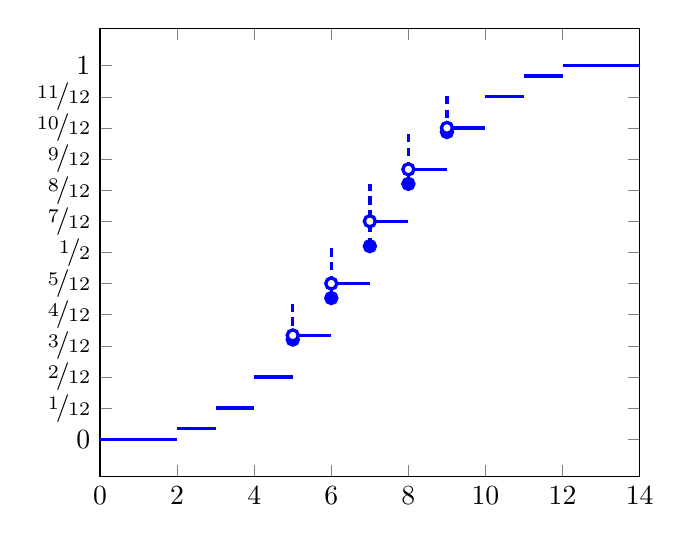
\begin{tikzpicture}
		\begin{axis}[
			jump mark left,
			ymin=-0.1,ymax=1.1,
			xmin=0, xmax=14,
			discontinuous,
			every axis plot/.style={very thick},			
			ytick={0.0,0.083,.166667,0.25,0.333,0.416,0.5,0.583,0.666,0.75,0.833,0.916,1.0},
			yticklabels={$0$, $\nicefrac{1}{12}$,$\nicefrac{2}{12}$,$\nicefrac{3}{12}$,$\nicefrac{4}{12}$,
				$\nicefrac{5}{12}$,$\nicefrac{1}{2}$,$\nicefrac{7}{12}$,$\nicefrac{8}{12}$,
				$\nicefrac{9}{12}$,$\nicefrac{10}{12}$,$\nicefrac{11}{12}$,$1$},
			table/create on use/cumulative distribution/.style=
				{create col/expr={\pgfmathaccuma + \thisrow{f(x)}}}
	]


			%TODO data is here - list the probabilities of each possible value of x
			\addplot [blue] table [y=cumulative distribution]{
				x f(x)
				0 0
				1 0
				2 1/36
				3 2/36
				4 3/36
				5 4/36
				6 5/36
				7 6/36
				8 5/36
				9 4/36
				10 3/36
				11 2/36
				12 1/36
				13 0
				14 0
			};
		\end{axis}
	\end{tikzpicture}
\end{document}
